\documentclass[]{BasiliskReportMemo}
\usepackage{AVS}

\newcommand{\submiterInstitute}{Autonomous Vehicle Simulation (AVS) Laboratory,\\ University of Colorado}

\newcommand{\ModuleName}{MRP\_Steering}
\newcommand{\subject}{MRP Steering ADCS Control Module}
\newcommand{\status}{Initial Documentation}
\newcommand{\preparer}{H. Schaub}
\newcommand{\summary}{This module uses the MRP Steering control logic to determine the ADCS control torque vector $\bm L_{r}$.}


\begin{document}


\makeCover


%
%	enter the revision documentation here
%	to add more lines, copy the table entry and the \hline, and paste after the current entry.
%
\pagestyle{empty}
{\renewcommand{\arraystretch}{2}
\noindent
\begin{longtable}{|p{0.5in}|p{4.5in}|p{1.14in}|}
\hline
{\bfseries Rev}: & {\bfseries Change Description} & {\bfseries By} \\
\hline
Draft & Initial Documentation Draft & H. Schaub \\
0.1 & Updated the sign definition of $\bm L_{r}$ & H. Schaub \\
\hline

\end{longtable}
}

\newpage
\setcounter{page}{1}
\pagestyle{fancy}

\tableofcontents
~\\ \hrule ~\\



\section{Initialization}
Simply call the module reset function prior to using this control module.  This will reset the prior function call time variable, and reset the attitude error integral measure.  The control update period $\Delta t$ is evaluated automatically.  


\section{Steering Law Goals}
This technical note develops a new MRP based steering law that drives a body frame \frameDefinition{B} towards a time varying reference frame \frameDefinition{R}. The inertial frame is given by \frameDefinition{N}.   The RW coordinate frame is given by $\mathcal{W_{i}}:\{ \hat{\bm g}_{s_{i}}, \hat{\bm g}_{t_{i}}, \hat{\bm g}_{g_{i}} \}$.  The   Using MRPs, the overall control goal is 
\begin{equation}
	\label{eq:MS:1}
	\bm\sigma_{\mathcal{B}/\mathcal{R}} \rightarrow 0
\end{equation}
The reference frame orientation $\bm \sigma_{\mathcal{R}/\mathcal{N}}$, angular velocity $\bm\omega_{\mathcal{R}/\mathcal{N}}$ and inertial angular acceleration $\dot{\bm \omega}_{\mathcal{R}/\mathcal{N}}$ are assumed to be known. 

The rotational equations of motion of a rigid spacecraft with $N$ Reaction Wheels (RWs) attached are given by\cite{schaub}
\begin{equation}
	\label{eq:MS:2}
	[I_{RW}] \dot{\bm \omega} = - [\tilde{\bm \omega}] \left( 
	[I_{RW}] \bm\omega + [G_{s}] \bm h_{s} 
	\right) - [G_{s}] \bm u_{s} + \bm L
\end{equation}
where  the inertia tensor $[I_{RW}]$ is defined as
\begin{equation}
	\label{eq:MS:3}
	[I_{RW}] = [I_{s}] + \sum_{i=1}^{N} \left (J_{t_{i}} \hat{\bm g}_{t_{i}} \hat{\bm g}_{t_{i}}^{T} + J_{g_{i}} \hat{\bm g}_{g_{i}} \hat{\bm g}_{g_{i}}^{T}
	\right)
\end{equation}
The spacecraft inertial without the $N$ RWs is $[I_{s}]$, while $J_{s_{i}}$, $J_{t_{i}}$ and $J_{g_{i}}$ are the RW inertias about the body fixed RW axis $\hat{\bm g}_{s_{i}}$ (RW spin axis), $\hat{\bm g}_{t_{i}}$ and $\hat{\bm g}_{g_{i}}$.  The $3\times N$ projection matrix $[G_{s}]$ is then defined as
\begin{equation}
	\label{eq:MS:4}
	[G_{s}] = \begin{bmatrix}
		\cdots \leftexp{B}{\hat{\bm g}}_{s_{i}} \cdots
	\end{bmatrix}
\end{equation}
The RW inertial angular momentum vector $\bm h_{s}$ is defined as
\begin{equation}
	\label{eq:MS:5}
	h_{s_{i}} = J_{s_{i}} (\omega_{s_{i}} + \Omega_{i})
\end{equation}
Here $\Omega_{i}$ is the $i^{\text{th}}$ RW spin relative to the spacecraft, and the body angular velocity is written in terms of body and RW frame components as
\begin{equation}
	\label{eq:MS:6}
	\bm\omega = \omega_{1} \hat{\bm b}_{1} + \omega_{2} \hat{\bm b}_{2} + \omega_{3} \hat{\bm b}_{3}
	= \omega_{s_{i}} \hat{\bm g}_{s_{i}} +  \omega_{t_{i}} \hat{\bm g}_{t_{i}} +  \omega_{g_{i}} \hat{\bm g}_{g_{i}}
\end{equation}









\section{MRP Steering Law}
\subsection{Steering Law Stability Requirement}
As is commonly done in robotic applications where the steering laws are of the form $\dot{\bm x} = \bm u$, this section derives a kinematic based attitude steering law.  Let us consider the simple Lyapunov candidate function\cite{Tsiotras:1994lr,schaub}
\begin{equation}
	\label{eq:MS:7}
	V ( \bm\sigma_{\mathcal{B}/\mathcal{R}} ) = 2 \ln \left ( 1 + \bm\sigma_{\mathcal{B}/\mathcal{R}} ^{T} \bm\sigma_{\mathcal{B}/\mathcal{R}} \right)
\end{equation}
in terms of the MRP attitude tracking error $\bm\sigma_{\mathcal{B}/\mathcal{R}}$.  Using the MRP differential kinematic equations
\begin{equation}
	\label{eq:MS:8}
	\dot{\bm\sigma}_{\mathcal{B}/\mathcal{R}} = \frac{1}{4}[B(\bm\sigma_{\mathcal{B}/\mathcal{R}})] \leftexp{B}{\bm\omega}_{\mathcal{B}/\mathcal{R}}
	= \frac{1}{4} \left[
	(1-\sigma_{\mathcal{B}/\mathcal{R}}^{2})[I_{3\times 3} + 2 [\tilde{\bm\sigma}_{\mathcal{B}/\mathcal{R}}] + 2 \bm\sigma_{\mathcal{B}/\mathcal{R}} \bm\sigma_{\mathcal{B}/\mathcal{R}}^{T}
	\right] \leftexp{B}{\bm\omega}_{\mathcal{B}/\mathcal{R}}
\end{equation}
where $\sigma_{\mathcal{B}/\mathcal{R}}^{2} = \bm\sigma_{\mathcal{B}/\mathcal{R}}^{T} \bm\sigma_{\mathcal{B}/\mathcal{R}}$, the time derivative of $V$ is
\begin{equation}
	\label{eq:MS:9}
	\dot V =\bm \sigma_{\mathcal{B}/\mathcal{R}}^{T} \left(  \leftexp{B}{ \bm\omega}_{\mathcal{B}/\mathcal{R}}  \right)
\end{equation}

To create a kinematic steering law, let ${\mathcal{B}}^{\ast}$ be the desired body orientation, and $\bm\omega_{{\mathcal{B}}^{\ast}/\mathcal{R}}$ be the desired angular velocity vector of this body orientation relative to the reference frame $\mathcal{R}$.  The steering law requires an algorithm for the desired body rates $\bm\omega_{{\mathcal{B}}^{\ast}/\mathcal{R}}$  relative to the reference frame make $\dot V$ in Eq.~\eqref{eq:MS:9} negative definite.  For this purpose, let us select
\begin{equation}
	\label{eq:MS:10}
	\leftexp{B}{\bm\omega}_{{\mathcal{B}}^{\ast}/\mathcal{R}} = - \bm f(\bm\sigma_{\mathcal{B}/\mathcal{R}})
\end{equation}
where $\bm f(\bm\sigma)$ is an even function such that 
\begin{equation}
	\label{eq:MS:11}
	\bm \sigma ^{T} \bm f(\bm \sigma) > 0
\end{equation}
The Lyapunov rate simplifies to the negative definite expression:
\begin{equation}
	\label{eq:MS:12}
	\dot V = -  \bm \sigma_{\mathcal{B}/\mathcal{R}}^{T} \bm f(\bm \sigma_{\mathcal{B}/\mathcal{R}}) < 0
\end{equation}



\subsection{Saturated  MRP Steering Law}
A very simple example would be to set
\begin{equation}
	\label{eq:MS:13}
	\bm f (\bm \sigma_{\mathcal{B}/\mathcal{R}}) =  K_{1} \bm \sigma_{\mathcal{B}/\mathcal{R}}
\end{equation}
where $K_{1}>0$.  
This yields a kinematic control where the desired body rates are proportional to the MRP attitude error measure.  If the rate should saturate, then $\bm f()$ could be defined as
\begin{equation}
	\label{eq:MS:14}
	\bm f(\bm \sigma_{\mathcal{B}/\mathcal{R}}) = \begin{cases}
		K_{1} \sigma_{i} 		&\text{if } |K_{1} \sigma_{i}| \le \omega_{\text{max}} \\
		\omega_{\text{max}} \text{sgn}(\sigma_{i}) &\text{if } |K_{1} \sigma_{i}| > \omega_{\text{max}}
	\end{cases}
\end{equation}
where
$$
	\bm\sigma_{\mathcal{B}/\mathcal{R}} = (\sigma_{1}, \sigma_{2}, \sigma_{3})^{T}
$$
A smoothly saturating function is given by
\begin{equation}
	\label{eq:MS:15}
	\bm f(\bm \sigma_{\mathcal{B}/\mathcal{R}}) = \arctan \left(
		\bm \sigma_{\mathcal{B}/\mathcal{R}} \frac{K_{1} \pi}{2  \omega_{\text{max}}}
	\right) \frac{2 \omega_{\text{max}}}{\pi}
\end{equation}
where
\begin{equation}
	\label{eq:MS:15.0}
	\bm f(\bm\sigma_{\mathcal{B}/\mathcal{R}}) = \begin{pmatrix}
		f(\sigma_{1})\\ f(\sigma_{2})\\ f(\sigma_{3})
		\end{pmatrix}
\end{equation}
Here as $\sigma_{i} \rightarrow \infty$ then the function $f$ smoothly converges to the maximum speed rate $\pm  \omega_{\text{max}}$.   For small $|\bm \sigma_{\mathcal{B}/\mathcal{R}}|$, this function linearizes to
\begin{equation}
	\bm f(\bm \sigma_{\mathcal{B}/\mathcal{R}}) \approx K_{1} \bm \sigma_{\mathcal{B}/\mathcal{R}} + \text{ H.O.T}
\end{equation}

If the MRP shadow set parameters are used to avoid the MRP singularity at 360\dg, then $|\bm \sigma_{\mathcal{B}/\mathcal{R}}|$ is upper limited by 1.  To control how rapidly the rate commands approach the $\omega_{\text{max}}$ limit, Eq.~\eqref{eq:MS:15} is modified to include a cubic term:
\begin{equation}
	\label{eq:MS:15.1}
	 f( \sigma_{i}) = \arctan \left(
		(K_{1} \sigma_{i} +K_{3} \sigma_{i}^{3}) \frac{ \pi}{2  \omega_{\text{max}}}
	\right) \frac{2 \omega_{\text{max}}}{\pi}
\end{equation}
The order of the polynomial must be odd to keep $\bm f()$ an even function.  A nice feature of Eq.~\eqref{eq:MS:15.1} is that the control rate is saturated individually about each axis.  If the smoothing component is removed to reduce this to a bang-band rate control, then this would yield a Lyapunov optimal control which minimizes $\dot V$ subject to the allowable rate constraint $\omega_{\text{max}}$.

\begin{figure}[tb]
	\centering
	\subfigure[$\omega_{\text{max}}$ dependency with $K_{1} = 0.1$, $K_{3} = 1$]
	{\label{fig:fSigmaOptionsA} 
	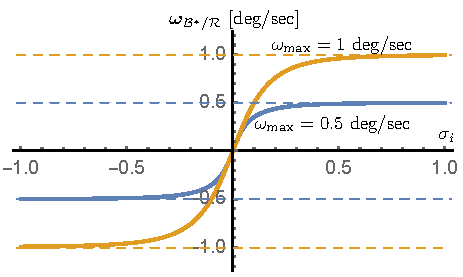
\includegraphics[]{Figures/fSigmaOptionsA}}  
	\subfigure[$K_{1}$ dependency with $\omega_{\text{max}}  = 1{\dg}/s$, $K_{3} = 1$]
	{\label{fig:fSigmaOptionsB}
	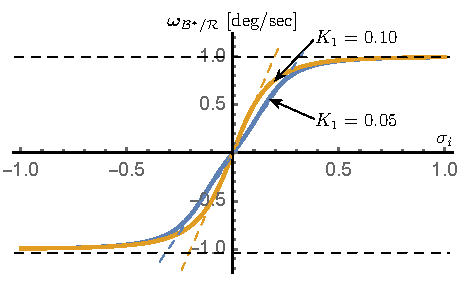
\includegraphics[]{Figures/fSigmaOptionsB}}
	\\
	\subfigure[$K_{3}$ dependency with $\omega_{\text{max}}  = 1{\dg}/s$, $K_{1} = 0.1$]
	{\label{fig:fSigmaOptionsC}
	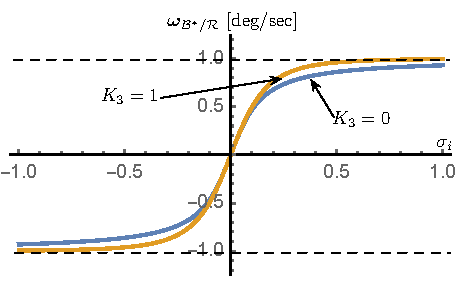
\includegraphics[]{Figures/fSigmaOptionsC}} 
	\caption{Illustrations of MRP Steering Parameters Influence.}
	\label{fig:fSigmaOptions}
\end{figure}

Figure~\ref{fig:fSigmaOptions} illustrates how the parameters $\omega_{\text{max}}$, $K_{1}$ and $K_{3}$ impact the steering law behavior.  The maximum steering law rate commands are easily set through the $\omega_{\text{max}}$ parameters.  The gain $K_{1}$ controls the linear stiffness when the attitude errors have become small, while $K_{3}$ controls how rapidly the steering law approaches the speed command limit.

The required velocity servo loop design is aided by knowing the body-frame derivative of $\leftexp{B}{\bm\omega}_{{\mathcal{B}}^{\ast}/\mathcal{R}}$ to implement a feed-forward components.  Using the $\bm f()$ function definition in Eq.~\eqref{eq:MS:15.0}, this requires the time derivatives of $f(\sigma_{i})$.  
\begin{equation}
	\frac{\leftexp{B}{\D (\leftexp{B}{\bm\omega}_{{\mathcal{B}}^{\ast}/\mathcal{R}} ) }}{\D t} =
	{\bm\omega}_{{\mathcal{B}}^{\ast}/\mathcal{R}} '
	= - \frac{\partial \bm f}{\partial \bm \sigma_{{\mathcal{B}}^{\ast}/\mathcal{R}}} \dot{\bm \sigma}_{{\mathcal{B}}^{\ast}/\mathcal{R}}
	= - \begin{pmatrix}
		\frac{\partial  f}{\partial  \sigma_{1}} \dot{ \sigma}_{1} \\
		\frac{\partial  f}{\partial  \sigma_{2}} \dot{ \sigma}_{2} \\
		\frac{\partial  f}{\partial  \sigma_{3}} \dot{ \sigma}_{3} 
	\end{pmatrix}
\end{equation}
where
\begin{equation}
	\dot{\bm\sigma}	_{{\mathcal{B}}^{\ast}/\mathcal{R}} = 
	\begin{pmatrix}
		\dot\sigma_{1}\\
		\dot\sigma_{2}\\
		\dot\sigma_{3}
	\end{pmatrix} = 
	 \frac{1}{4}[B(\bm\sigma_{{\mathcal{B}}^{\ast}/\mathcal{R}})] 
	\leftexp{B}{\bm\omega}_{{\mathcal{B}}^{\ast}/\mathcal{R}}
\end{equation}
Using the general $f()$ definition in Eq.~\eqref{eq:MS:15.1}, its sensitivity with respect to $\sigma_{i}$ is
\begin{equation}
	\frac{
		\partial f
	}{
		\partial \sigma_{i}
	} = 
	\frac{
	(K_{1}  + 3 K_{3} \sigma_{i}^{2})
	}{
	1+(K_{1}\sigma_{i} + K_{3} \sigma_{i}^{3})^{2} \left(\frac{\pi}{2 \omega_{\text{max}}}\right)^{2}
	}
\end{equation}





















%\subsection{Principal Angle Steering Law}
%Consider the following saturation function $\bm f(\bm \sigma_{\mathcal{B}/\mathcal{R}})$ which is colinear with the principal rotation axis  $\hat{\bm e}_{\mathcal{B}/\mathcal{R}}$, and the magnitude scales uniformly with the principal rotation angle $\phi_{\mathcal{B}/\mathcal{R}}$:
%\begin{equation}
%	\label{eq:MS:16}
%	\bm f (\bm \sigma_{\mathcal{B}/\mathcal{R}}) = \hat{\bm e}_{\mathcal{B}/\mathcal{R}} f(\phi_{\mathcal{B}/\mathcal{R}})
%\end{equation}
%The scalar function $f(\phi_{\mathcal{B}/\mathcal{R}})$ is an even function where $f(\phi_{\mathcal{B}/\mathcal{R}})\phi_{\mathcal{B}/\mathcal{R}} \ge 0$.  Note that $\hat{\bm e}_{\mathcal{B}/\mathcal{R}}$ is ill-defined for a zero principal rotation angle.  This saturation function will need a check to avoid numerical issues right at the zero angle condition.
%
%Using the MRP definition in terms of principal rotation angle and axis
%\begin{equation}
%	\label{eq:MS:17}
%	\bm \sigma_{\mathcal{B}/\mathcal{R}} = \hat{\bm e}_{\mathcal{B}/\mathcal{R}} \tan\left(\frac{\phi_{\mathcal{B}/\mathcal{R}}}{4}\right)
%\end{equation}
%and substituting into Eq.~\eqref{eq:MS:12}, the Lyapunov rate is for this case
%\begin{equation}
%	\label{eq:MS:18}
%	\dot V =  -  \bm \sigma_{\mathcal{B}/\mathcal{R}}^{T} \bm f(\bm \sigma_{\mathcal{B}/\mathcal{R}})
%	= -   \tan\left(\frac{\phi_{\mathcal{B}/\mathcal{R}}}{4}\right) \hat{\bm e}_{\mathcal{B}/\mathcal{R}}^{T} \hat{\bm e}_{\mathcal{B}/\mathcal{R}} f(\phi_{\mathcal{B}/\mathcal{R}})
%	= -   \tan\left(\frac{\phi_{\mathcal{B}/\mathcal{R}}}{4}\right)f(\phi_{\mathcal{B}/\mathcal{R}}) < 0
%\end{equation}
%This $\dot V$ is negative definite in terms of the attitude error, thus yielding asymptotic convergence.  The saturation function in Eq.~\eqref{eq:MS:16} has the convenient property that the resulting steering law employs an eigenaxis rotation towards the desired reference orientation.  In contrast, the smoothing function in Eq.~\eqref{eq:MS:15} saturates the MRP components individually, deviating fro man eigen-axis rotation.  The benefit of the later is that small errors are reduced quickly, thus reducing the overall tracking error quicker.  The benefit of the eigenaxis approach is that the closed-loop attitude path towards the reference is more predictable.  
%
%
%
%\begin{figure}[tb]
%	\centering
%	\subfigure[$\omega_{\text{max}}$ dependency with $K_{1} = 0.034$, $K_{3} = 0.034$]
%	{\label{fig:fOptionsA} 
%	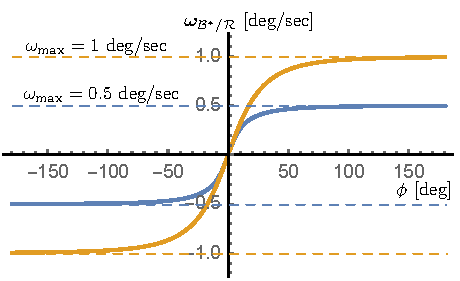
\includegraphics[]{Figures/fOptionsA}}  
%	\subfigure[$K_{1}$ dependency with $\omega_{\text{max}}  = 1{\dg}/s$, $K_{3} = 0.034$]
%	{\label{fig:fOptionsB}
%	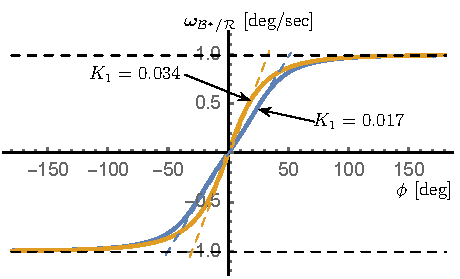
\includegraphics[]{Figures/fOptionsB}}
%	\\
%	\subfigure[$K_{3}$ dependency with $\omega_{\text{max}}  = 1{\dg}/s$, $K_{1} = 0.034$]
%	{\label{fig:fOptionsC}
%	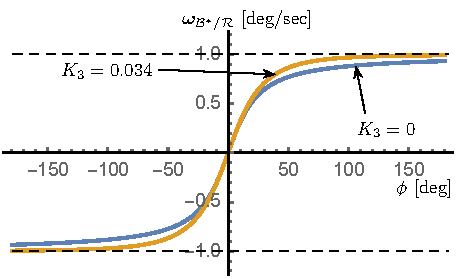
\includegraphics[]{Figures/fOptionsC}} 
%	\caption{Illustrations of Principal Angle Steering Parameters Influence.}
%	\label{fig:fOptions}
%\end{figure}
%
%Consider the $f(\bm \phi_{\mathcal{B}/\mathcal{R}})$ function given by:
%\begin{equation}
%	\label{eq:MS:19}
%	f(\phi_{\mathcal{B}/\mathcal{R}}) = 
%	\arctan \left(
%		(K_{1}\phi_{\mathcal{B}/\mathcal{R}} + K_{3} \phi_{\mathcal{B}/\mathcal{R}}^{3}) \frac{\pi}{2 \omega_{\text{max}}}
%	\right) \frac{2 \omega_{\text{max}}}{\pi}
%\end{equation}
%The linear approximation of this function is
%\begin{equation}
%	f(\phi_{\mathcal{B}/\mathcal{R}}) \approx K_{1} \phi_{\mathcal{B}/\mathcal{R}} + \text{ H.O.T}
%\end{equation}
%
%The resulting attitude steering law is of the form:
%\begin{equation}
%	\label{eq:MS:20}
%	\bm\omega_{{\mathcal{B}}^{\ast}/\mathcal{R}} = -  \hat{\bm e}_{\mathcal{B}/\mathcal{R}} 
%	\arctan \left(
%		(K_{1}\phi_{\mathcal{B}/\mathcal{R}} + K_{3} \phi_{\mathcal{B}/\mathcal{R}}^{3}) \frac{\pi}{2 \omega_{\text{max}}}
%	\right) \frac{2 \omega_{\text{max}}}{\pi}
%\end{equation}
%The impacts of the steering law gains $\omega_{\text{max}}$, $K_{1}$ and $K_{3}$ are illustrated in Figure~\ref{fig:fOptions}.  As the function $f(\phi)$  returns a value of $\pm \omega_{\text{max}}$ as $\phi\rightarrow \infty$, the gain $\omega_{\text{max}}$ determines the maximum rate limit that the steering law with request.  This is illustrated in Figure~\ref{fig:fOptionsA} where reducing the $\omega_{\text{max}}$ value by a factor of 2 results in half of the asymptotic rate command.  
%
%The parameter $K_{1}$ determines the final  pointing stiffness, and determines the final exponential convergence of the attitude pointing error as illustrated in Figure~\ref{fig:fOptionsB}.  Increasing this value results in faster final convergence once the principal rotation error has reduced past the saturated $f(\phi)$ function region.  
%
%Finally, the higher order $\phi$ polynomial is provided to cause the $f(\phi)$ function to saturate more quickly.  Setting $K_{3} $ = 0.034 in Figure~\ref{fig:fOptionsC} doesn't change the initial slope of the rate command, but impacts how quickly the rates saturate on the maximum speed command.
%
%
%Because $\hat{\bm e}_{\mathcal{B}/\mathcal{R}}'= 0$, the body relative time derivative of the steering control is
%\begin{equation}
%	\label{eq:MS:28}
%	\frac{\leftexp{B}{\D (\leftexp{B}{\bm\omega}_{{\mathcal{B}}^{\ast}/\mathcal{R}} ) }}{\D t} =
%	{\bm\omega}_{{\mathcal{B}}^{\ast}/\mathcal{R}} '
%	= - \hat{\bm e}_{\mathcal{B}/\mathcal{R}} \frac{\partial f(\phi_{\mathcal{B}/\mathcal{R}})}{\partial \phi_{\mathcal{B}/\mathcal{R}}} \dot\phi_{\mathcal{B}/\mathcal{R}}
%\end{equation}
%The $f()$ function sensitivity is
%\begin{equation}
%	\frac{
%		\partial f
%	}{
%		\partial \phi_{\mathcal{B}/\mathcal{R}}
%	} = 
%	\frac{
%	(K_{1}  + 3 K_{3} \phi_{\mathcal{B}/\mathcal{R}}^{2})
%	}{
%	1+(K_{1}\phi_{\mathcal{B}/\mathcal{R}} + K_{3} \phi_{\mathcal{B}/\mathcal{R}}^{3})^{2} \left(\frac{\pi}{2 \omega_{\text{max}}}\right)^{2}
%	}
%\end{equation}
%The principal rotation angle time derivative is given by\cite{hughes}
%\begin{equation}
%	\label{eq:MS:30}
%	\dot\phi_{\mathcal{B}/\mathcal{R}} = \hat{\bm e}_{\mathcal{B}/\mathcal{R}}^{T} 
%	\leftexp{B}{\bm\omega}_{{\mathcal{B}}^{\ast}/\mathcal{R}} 
%\end{equation}
%Substituting Eqs.~\eqref{eq:MS:10} and \eqref{eq:MS:30} into Eq.~\eqref{eq:MS:28} yields
%\begin{align}
%	{\bm\omega}_{{\mathcal{B}}^{\ast}/\mathcal{R}} '
%	&= - \hat{\bm e}_{\mathcal{B}/\mathcal{R}} \frac{\partial f(\phi_{\mathcal{B}/\mathcal{R}})}{\partial \phi_{\mathcal{B}/\mathcal{R}}} 
%	\left( \hat{\bm e}_{\mathcal{B}/\mathcal{R}}^{T} 
%	\leftexp{B}{\bm\omega}_{{\mathcal{B}}^{\ast}/\mathcal{R}}  \right)
%	\nonumber \\
%	&= -
%	 \hat{\bm e}_{\mathcal{B}/\mathcal{R}} \frac{\partial f(\phi_{\mathcal{B}/\mathcal{R}})}{\partial \phi_{\mathcal{B}/\mathcal{R}}} 
%	 \left( \hat{\bm e}_{\mathcal{B}/\mathcal{R}}^{T} 
%	 (-\hat{\bm e}_{\mathcal{B}/\mathcal{R}} f(\phi_{\mathcal{B}/\mathcal{R}}))
%	\right)
%	\nonumber \\
%	&= \hat{\bm e}_{\mathcal{B}/\mathcal{R}} \frac{\partial f(\phi_{\mathcal{B}/\mathcal{R}})}{\partial \phi_{\mathcal{B}/\mathcal{R}}} 
%	  f(\phi_{\mathcal{B}/\mathcal{R}}))
%\end{align}	
%














\section{Angular Velocity Servo Sub-System}
To implement the kinematic steering control, a servo sub-system must be included which will produce the required torques to make the actual body rates track the desired body rates.  The angular velocity tracking error vector is defined as
\begin{equation}
	\label{eq:MS:32}
	\delta \bm \omega = \bm\omega_{\mathcal{B}/\mathcal{B}^{\ast}} = \bm\omega_{\mathcal{B}/\mathcal{N}} - \bm\omega_{\mathcal{B}^{\ast}/\mathcal{N}}
\end{equation}
where the $\mathcal{B}^{\ast}$ frame is the desired body frame from the kinematic steering law.  Note that
\begin{equation}
	 \bm\omega_{\mathcal{B}^{\ast}/\mathcal{N}} =  \bm\omega_{\mathcal{B}^{\ast}/\mathcal{R}} +  \bm\omega_{\mathcal{R}/\mathcal{N}}
\end{equation}
where $\bm\omega_{\mathcal{R}/\mathcal{N}}$ is obtained from the attitude navigation solution, and $ \bm\omega_{\mathcal{B}^{\ast}/\mathcal{R}}$ is the kinematic steering rate command.  To create a rate-servo system that is robust to unmodeld torque biases, the state $\bm z$ is defined as:
\begin{equation}
	\label{eq:MS:34}
	\bm z = \int_{t_{0}}^{t_{f}} \leftexp{B}{ \delta\bm\omega}\ \D t
\end{equation}

The rate servo Lyapunov function is defined as 
\begin{equation}
	\label{eq:MS:35}
	V_{\bm\omega}(\delta\bm\omega, \bm z) = \frac{1}{2} \delta\bm\omega ^{T} [I_{\text{RW}}] \delta\bm\omega + \frac{1}{2} \bm z ^{T} [K_{I}] \bm z
\end{equation}
where the vector $\delta\bm\omega$ and tensor $[I_{\text{RW}}]$ are assumed to be given in body frame components, $[K_{i}]$ is a symmetric positive definite matrix.  The time derivative of this Lyapunov function is
\begin{equation}
	\label{eq:MS:36}
	\dot V_{\bm\omega} = \delta\bm\omega^{T} \left(
		[I_{\text{RW}}] \delta\bm\omega' + [K_{I}] \bm z
	\right)
\end{equation}
Using the identities ${\bm\omega}_{\mathcal{B}/\mathcal{N}}' = \dot{\bm\omega}_{\mathcal{B}/\mathcal{N}}$ and $ \bm\omega_{\mathcal{R}/\mathcal{N}}' =  \dot{\bm\omega}_{\mathcal{R}/\mathcal{N}} -  {\bm\omega}_{\mathcal{B}/\mathcal{N}} \times  \bm\omega_{\mathcal{R}/\mathcal{N}}$,\cite{schaub} the body frame derivative of $\delta \bm\omega$ is
\begin{equation}
	\label{eq:MS:37}
	\delta\bm \omega '= \dot{\bm\omega}_{\mathcal{B}/\mathcal{N}} - \bm\omega_{\mathcal{B}^{\ast}/\mathcal{R}} ' -  \dot{\bm\omega}_{\mathcal{R}/\mathcal{N}} +  {\bm\omega}_{\mathcal{B}/\mathcal{N}} \times  \bm\omega_{\mathcal{R}/\mathcal{N}}
\end{equation}
Substituting Eqs.~\eqref{eq:MS:2} and \eqref{eq:MS:37} into the $\dot V_{\bm\omega}$ expression in Eq.~\eqref{eq:MS:36} yields
\begin{multline}
	\label{eq:MS:38}
	\dot V_{\bm\omega} = \delta\bm\omega^{T} \Big(
		- [\tilde{\bm \omega}_{\mathcal{B}/\mathcal{N}}] \left( 
	[I_{RW}] \bm\omega_{\mathcal{B}/\mathcal{N}} + [G_{s}] \bm h_{s} 
	\right) - [G_{s}] \bm u_{s} + \bm L + [K_{I}] \bm z
	\\
	- [I_{\text{RW}}](\bm\omega_{\mathcal{B}^{\ast}/\mathcal{R}} ' +  \dot{\bm\omega}_{\mathcal{R}/\mathcal{N}} - {\bm\omega}_{\mathcal{B}/\mathcal{N}} \times  \bm\omega_{\mathcal{R}/\mathcal{N}})
	\Big)
\end{multline}

%\begin{equation}
%	\label{eq:MS:39}
%	\dot V_{\bm\omega} = - \delta\bm\omega^{T} [P]\delta\bm\omega
%\end{equation}
Let $[P]^{T} = [P]>$ be a symmetric positive definite rate feedback gain matrix.  The servo rate feedback control is defined as
\begin{multline}
	\label{eq:MS:39}
	[G_{s}]\bm u_{s} = [P]\delta\bm\omega + [K_{I}]\bm z - [\tilde{\bm\omega}_{\mathcal{B}^{\ast}/\mathcal{N}}] 
	\left( [I_{\text{RW}}] \bm\omega_{\mathcal{B}/\mathcal{N}} + [G_{s}] \bm h_{s} \right)
	\\
	- [I_{\text{RW}}](\bm\omega_{\mathcal{B}^{\ast}/\mathcal{R}} ' +  \dot{\bm\omega}_{\mathcal{R}/\mathcal{N}} -  {\bm\omega}_{\mathcal{B}/\mathcal{N}} \times  \bm\omega_{\mathcal{R}/\mathcal{N}}) + \bm L
\end{multline}
Defining the right-hand-side as $\bm L_{r}$, this is rewritten in compact form as
\begin{equation}
	[G_{s}]\bm u_{s} = -\bm L_{r}
\end{equation}
The array of RW motor torques can be solved with the typical minimum norm inverse
\begin{equation}
	\bm u_{s} = [G_{s}]^{T}\left( [G_{s}][G_{s}]^{T}\right)^{-1} (- \bm L_{r})
\end{equation}


To analyze the stability of this rate servo control, the $[G_{s}]\bm u_{s}$ expression in Eq.~\eqref{eq:MS:39} is substituted into the Lyapunov rate expression in Eq.~\eqref{eq:MS:38}.
\begin{align}
	\label{eq:MS:42}
	\dot V_{\omega} &= \delta\bm\omega^{T} \Big(
		- [P]\delta\bm\omega - [\tilde{\bm \omega}_{\mathcal{B}/\mathcal{N}}] \left( 
	[I_{RW}] \bm\omega_{\mathcal{B}/\mathcal{N}} + [G_{s}] \bm h_{s} 
	\right) 
	+ [\tilde{\bm\omega}_{\mathcal{B}^{\ast}/\mathcal{N}}] 
	\left( [I_{\text{RW}}] \bm\omega_{\mathcal{B}/\mathcal{N}} + [G_{s}] \bm h_{s} \right)
	\Big ) 
	\nonumber \\
	&= \delta\bm\omega^{T} \Big( - [P]\delta\bm\omega
	- [\widetilde{\delta\bm \omega}] \left( 
	[I_{RW}] \bm\omega_{\mathcal{B}/\mathcal{N}} + [G_{s}] \bm h_{s} 
	\right) 
	\Big )
	\nonumber \\
	&= - \delta\bm\omega ^{T} [P] \delta\bm\omega < 0
\end{align}
Thus, in the absence of unmodeled torques, the servo control in Eq.~\eqref{eq:MS:39} is asymptotically stabilizing in rate tracking error $\delta\bm\omega$.  

Next, the servo robustness to unmodeled external torques is investigated.  Let us assume that the external torque vector $\bm L$ in Eq.~\eqref{eq:MS:2} only approximates the true external torque, and the unmodeled component is given by $\Delta \bm L$.  Substituting the true equations of motion and the same servo control in Eq.~\eqref{eq:MS:39} into the Lyapunov rate expression in Eq.~\eqref{eq:MS:36} leads to
\begin{equation}
	\label{eq:MS:43}
	\dot V_{\omega} = - \delta\bm\omega ^{T} [P] \delta\bm\omega - \delta\bm\omega ^{T} \Delta \bm L
\end{equation}
This $\dot V_{\omega}$ is no longer negative definite due to the underdetermined sign of the $\delta\bm\omega ^{T} \Delta \bm L$ components.  Equating the Lyapunov rates in Eqs.~\eqref{eq:MS:36} and \eqref{eq:MS:43} yields the following servo closed loop dynamics:
\begin{equation}
	\label{eq:MS:44}
	[I_{\text{RW}}]\delta\bm\omega' + [P]\delta\bm\omega + [K_{I}]\bm z = \Delta\bm L
\end{equation}
Assuming that $\Delta\bm L$ is either constant as seen by the body frame, or at least varies slowly, then taking a body-frame time derivative of Eq.~\eqref{eq:MS:44} is
\begin{equation}
	\label{eq:MS:45}
	[I_{\text{RW}}]\delta\bm\omega'' + [P]\delta\bm\omega' + [K_{I}]\delta \bm \omega = \Delta\bm L' \approx 0 	
\end{equation}
As $[I_{\text{RW}}]$, $[P]$ and $[K_{I}]$ are all symmetric positive definite matrices, these linear differential equations are stable, and $\delta\bm\omega\rightarrow0$ given that assumption that $\Delta\bm L' \approx 0$.  


\bibliographystyle{unsrt}   % Number the references.
\bibliography{references}   % Use references.bib to resolve the labels.




\end{document}
